% -*- latex -*-
%%%%%%%%%%%%%%%%%%%%%%%%%%%%%%%%%%%%%%%%%%%%%%%%%%%%%%%%%%%%%%%%
%%%%%%%%%%%%%%%%%%%%%%%%%%%%%%%%%%%%%%%%%%%%%%%%%%%%%%%%%%%%%%%%
%%%%
%%%% This text file is part of the source of 
%%%% `Parallel Programming in MPI and OpenMP'
%%%% by Victor Eijkhout, copyright 2012-2021
%%%%
%%%% mpi-intercomm.tex : about splitting communicators
%%%%
%%%%%%%%%%%%%%%%%%%%%%%%%%%%%%%%%%%%%%%%%%%%%%%%%%%%%%%%%%%%%%%%
%%%%%%%%%%%%%%%%%%%%%%%%%%%%%%%%%%%%%%%%%%%%%%%%%%%%%%%%%%%%%%%%

\Level 0 {Inter-communicators}
\label{sec:mpi-intercomm}

In several scenarios it may be desirable to have a way to communicate
between communicators. For instance, an application can have clearly
functionally separated modules (preprocessor, simulation,
postprocessor) that need to stream data pairwise. In another example,
dynamically spawned processes (section~\ref{sec:mpi-dynamic}) get
their own value of \indexmpishow{MPI_COMM_WORLD}, but still need to
communicate with the process(es) that spawned them. In this section we
will discuss the \indextermsubh{inter}{communicator} mechanism that
serves such use cases.

Communicating between disjoint communicators can of course be done by
having a
communicator that overlaps them, but this would be complicated: since
the `inter' communication happens in the overlap communicator, you
have to translate its ordering into those of the two worker
communicators. It would be easier to express messages directly in
terms of those communicators, and this is what happens in an
\indextermsubh{inter}{communicator}.

\begin{figure}[ht]
  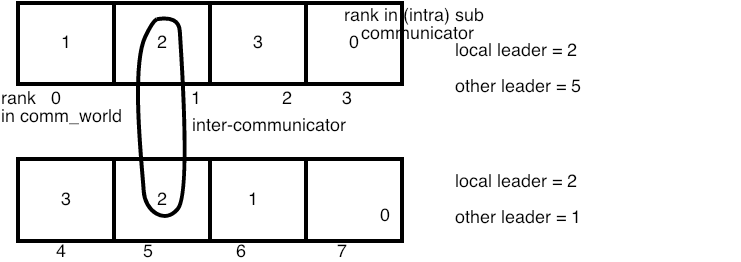
\includegraphics[scale=.6]{intercomm}
  \caption{Illustration of ranks in an inter-communicator setup}
  \label{fig:intercomm}
\end{figure}

A call to
\indexmpiref{MPI_Intercomm_create}
involves the following communicators:
\begin{itemize}
\item Two local communicators, which in this context are known as
  \indextermsubh{intra}{communicator}s: one process in each will act as
  the local leader, connected to the remote leader;
\item The \indextermsub{peer}{communicator}, often
  \indexmpishow{MPI_COMM_WORLD}, that contains the local
  communicators;
\item An \indextermsubdefh{inter}{communicator} that allows the leaders
  of the subcommunicators to communicate with the other subcommunicator.
\end{itemize}
Even though the intercommunicator connects only two proceses, it is
collective on the peer communicator.

\Level 1 {Inter-communicator point-to-point}

The local leaders can now communicate with each other.
\begin{itemize}
\item The sender specifies as target the local number of the other
  leader in the other sub-communicator;
\item Likewise, the receiver specifies as source the local number of
  the sender in its sub-communicator.
\end{itemize}
In one way, this design makes sense: processors are referred to in
their natural, local, numbering.
On the other hand, it means that each group needs to know how the
local ordering of the other group is arranged. Using a complicated
\lstinline{key} value makes this difficult.

\cverbatimsnippet[examples/mpi/c/intercomm.c]{intercomm-ptp}

\Level 1 {Inter-communicator collectives}

The intercommunicator can be used in collectives such as
a broadcast.

\begin{itemize}
\item In the sending group, the root process passes \indexmpishow{MPI_ROOT} as
  `root' value; all others use \indexmpishow{MPI_PROC_NULL}.
\item In the receiving group, all processes use a `root' value that is the
  rank of the root process in the root group. Note: this is not the
  global rank!
\end{itemize}
Gather and scatter behave similarly; the allgather is different: all
send buffers of group~A are concatenated in rank order, and places on
all processes of group~B.

Inter-communicators can be used if two groups of process work
asynchronously with respect to each other; another application is
fault tolerance (section~\ref{mpi:tolerant}).

\cverbatimsnippet[examples/mpi/c/intercomm.c]{intercomm-bcast}

\Level 1 {Inter-communicator querying}
\label{sec:mpi-inter-query}

Some of the operations you have seen before for
\indextermsubh{intra}{communicator}s behave differently with inter-communicator:
\begin{itemize}
\item \indexmpishow{MPI_Comm_size} returns the size of the local
  group, not the size of the inter-communicator.
\item \indexmpishow{MPI_Comm_rank} returns the rank in the local
  group.
\item \indexmpishow{MPI_Comm_group} returns the local group.
\end{itemize}

Spawned processes can find their parent communicator with
\indexmpiref{MPI_Comm_get_parent}
(see examples in section~\ref{sec:mpi-dynamic}).
On other processes this returns \indexmpishow{MPI_COMM_NULL}.

Test whether a communicator is intra or inter:
\indexmpiref{MPI_Comm_test_inter}.

\indexmpishow{MPI_Comm_compare} works for inter-communicators.

Processes connected through an intercommunicator can query
the size of the `other' communicator with
\indexmpiref{MPI_Comm_remote_size}.
The actual group can be obtained with
\indexmpiref{MPI_Comm_remote_group}.

Virtual topologies (chapter~\ref{ch:mpi-topo}) cannot be created with an intercommunicator.
To set up virtual topologies, first transform the intercommunicator to an
intracommunicator with the function
\indexmpiref{MPI_Intercomm_merge}.

